% Options for packages loaded elsewhere
\PassOptionsToPackage{unicode}{hyperref}
\PassOptionsToPackage{hyphens}{url}
%
\documentclass[
]{article}
\usepackage{amsmath,amssymb}
\usepackage{lmodern}
\usepackage{iftex}
\ifPDFTeX
  \usepackage[T1]{fontenc}
  \usepackage[utf8]{inputenc}
  \usepackage{textcomp} % provide euro and other symbols
\else % if luatex or xetex
  \usepackage{unicode-math}
  \defaultfontfeatures{Scale=MatchLowercase}
  \defaultfontfeatures[\rmfamily]{Ligatures=TeX,Scale=1}
\fi
% Use upquote if available, for straight quotes in verbatim environments
\IfFileExists{upquote.sty}{\usepackage{upquote}}{}
\IfFileExists{microtype.sty}{% use microtype if available
  \usepackage[]{microtype}
  \UseMicrotypeSet[protrusion]{basicmath} % disable protrusion for tt fonts
}{}
\makeatletter
\@ifundefined{KOMAClassName}{% if non-KOMA class
  \IfFileExists{parskip.sty}{%
    \usepackage{parskip}
  }{% else
    \setlength{\parindent}{0pt}
    \setlength{\parskip}{6pt plus 2pt minus 1pt}}
}{% if KOMA class
  \KOMAoptions{parskip=half}}
\makeatother
\usepackage{xcolor}
\usepackage[margin=1in]{geometry}
\usepackage{graphicx}
\makeatletter
\def\maxwidth{\ifdim\Gin@nat@width>\linewidth\linewidth\else\Gin@nat@width\fi}
\def\maxheight{\ifdim\Gin@nat@height>\textheight\textheight\else\Gin@nat@height\fi}
\makeatother
% Scale images if necessary, so that they will not overflow the page
% margins by default, and it is still possible to overwrite the defaults
% using explicit options in \includegraphics[width, height, ...]{}
\setkeys{Gin}{width=\maxwidth,height=\maxheight,keepaspectratio}
% Set default figure placement to htbp
\makeatletter
\def\fps@figure{htbp}
\makeatother
\setlength{\emergencystretch}{3em} % prevent overfull lines
\providecommand{\tightlist}{%
  \setlength{\itemsep}{0pt}\setlength{\parskip}{0pt}}
\setcounter{secnumdepth}{5}
\usepackage{booktabs,longtable,dcolumn} \usepackage{multirow,array} \usepackage{wrapfig,float} \floatplacement{figure}{H}
\ifLuaTeX
  \usepackage{selnolig}  % disable illegal ligatures
\fi
\IfFileExists{bookmark.sty}{\usepackage{bookmark}}{\usepackage{hyperref}}
\IfFileExists{xurl.sty}{\usepackage{xurl}}{} % add URL line breaks if available
\urlstyle{same} % disable monospaced font for URLs
\hypersetup{
  pdftitle={Matched Regressions QuickPay (2009-2012)},
  hidelinks,
  pdfcreator={LaTeX via pandoc}}

\title{Matched Regressions QuickPay (2009-2012)}
\author{}
\date{\vspace{-2.5em}Nov 22, 2022}

\begin{document}
\maketitle

\hypertarget{matching}{%
\section{Matching}\label{matching}}

Treatment and control groups matched exactly on three characteristics: -
Product or Service Code - Subagency - Type of pricing

\hypertarget{delays-over-time}{%
\section{Delays over Time}\label{delays-over-time}}

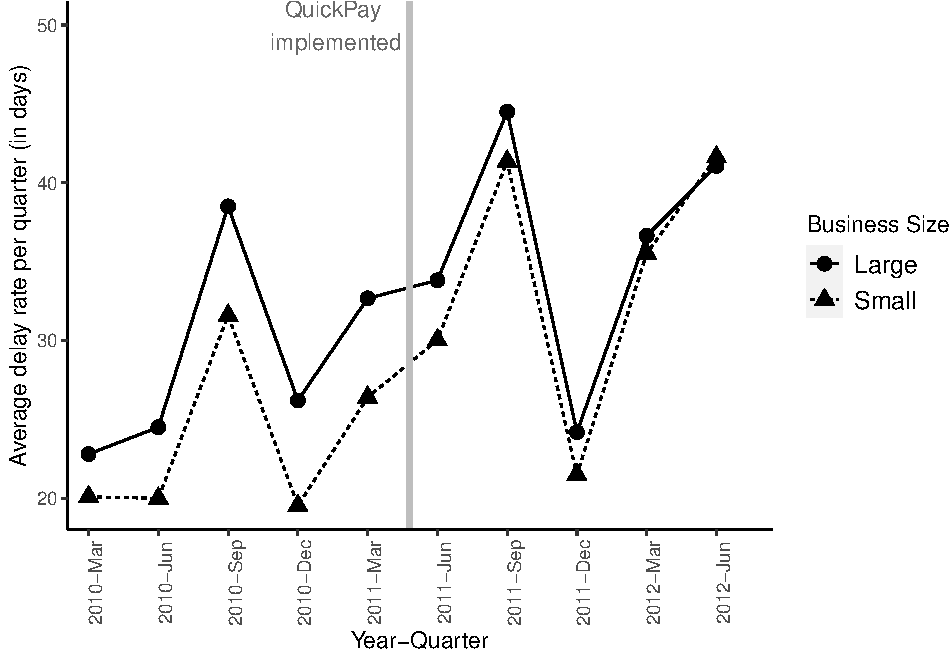
\includegraphics{qp_first_matched_files/figure-latex/plot-1.pdf}

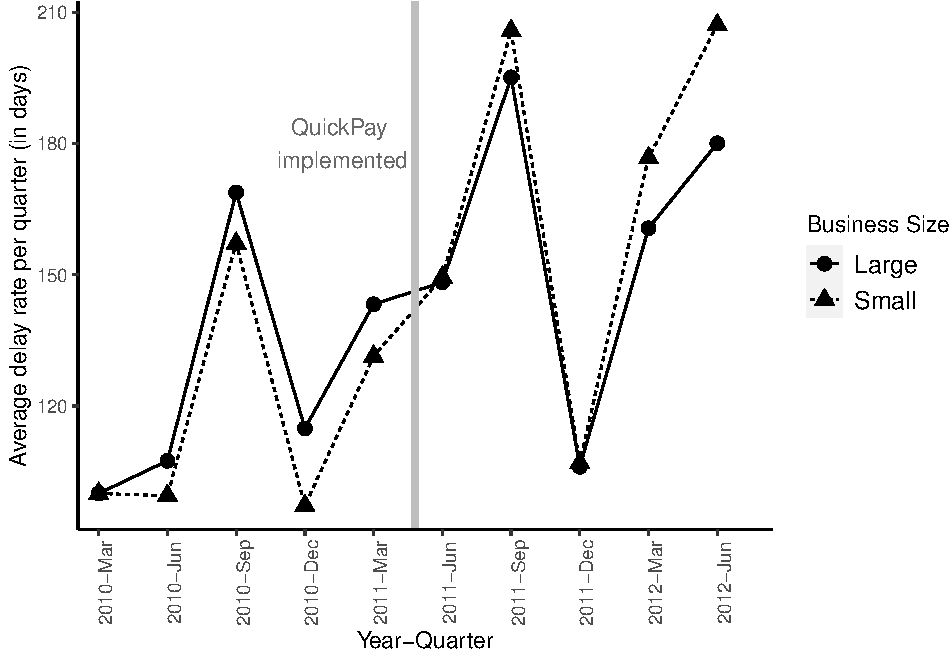
\includegraphics{qp_first_matched_files/figure-latex/normalized_plot-1.pdf}

\hypertarget{notation}{%
\section{Notation}\label{notation}}

\begin{itemize}
\tightlist
\item
  Project \(i\), Year-Quarter \(t\)
\item
  \(X_i\) denotes project level controls: initial duration, initial
  budget, number of offers received
\item
  \(\mu_t,\theta_{firm},\lambda_{task}\): Year-Quarter, Firm, and
  Product/Service code Fixed effects
\item
  All continuous variables are winsorized at the 5\% level
  \[ Treat_i = \begin{cases} 1, \text{ if project } i \text{ is a small business}\\
  0, \text{ otherwise} \end{cases}\]
  \[ Post_t = \begin{cases} 1, \text{ if year-quarter } t > \text{ April 27, 2011}\\
  0, \text{ otherwise} \end{cases}\]
\end{itemize}

\hypertarget{parallel-trends-test}{%
\section{Parallel Trends Test}\label{parallel-trends-test}}

Let \(Time\) denote \(q\)-th quarter since the beginning of time
horizon. For \(Post_t =0\), we run the following regression:
\[ DelayRate_{it} = \alpha+\beta_0 Treat_i + \beta_1 (Treat_i \times Time) + \beta_2 X_i + \mu_t + \theta_{firm} + \lambda_{task} +\epsilon_{it}\]
The coefficient of interest is \(\beta_1\). If this is significant, we
would find evidence of a linear time trend before quickpay
implementation -- violating the parallel trends assumption.

\begin{table}[H] \centering 
  \caption{Linear Time Trend Before QuickPay} 
  \label{} 
\small 
\begin{tabular}{@{\extracolsep{5pt}}lc} 
\\[-1.8ex]\hline 
\hline \\[-1.8ex] 
 & \multicolumn{1}{c}{\textit{Dependent variable:}} \\ 
\cline{2-2} 
\\[-1.8ex] & $DelayRate_{it}$ (in percentage) \\ 
\hline \\[-1.8ex] 
 $Treat_i$ & $-$2.70$^{***}$ \\ 
  & (0.71) \\ 
  & \\ 
 $Treat_i \times Time$ & 0.34$^{*}$ \\ 
  & (0.17) \\ 
  & \\ 
\hline \\[-1.8ex] 
Fixed effects & Firm, Task, and Year-Quarter \\ 
Controls & Budget, Duration, Bids, Project Age \\ 
Observations & 39,422 \\ 
R$^{2}$ & 0.15 \\ 
Adjusted R$^{2}$ & 0.14 \\ 
\hline 
\hline \\[-1.8ex] 
\textit{Note:}  & \multicolumn{1}{r}{$^{*}$p$<$0.1; $^{**}$p$<$0.05; $^{***}$p$<$0.01} \\ 
 & \multicolumn{1}{r}{Each observation is a project-quarter.} \\ 
 & \multicolumn{1}{r}{SEs are robust and clustered at the project level.} \\ 
 & \multicolumn{1}{r}{Observations are for quarters before quickpay.} \\ 
\end{tabular} 
\end{table}

\hypertarget{baseline-regressions}{%
\section{Baseline Regressions}\label{baseline-regressions}}

\[ DelayRate_{it} = \alpha+\beta_0 Treat_i + \beta_1 Post_t + \beta_2 (Treat_i \times Post_t) + \epsilon_{it}\]

\[ \begin{aligned} DelayRate_{it} &=& \alpha+\beta_0 Treat_i + \beta_1 Post_t + \beta_2 (Treat_i \times Post_t)\\
&+&  X_i + (Post_t \times X_i) + \mu_t + \theta_{firm} + \lambda_{task}+ \epsilon_{it}
\end{aligned}\]

\begin{table}[H] \centering 
  \caption{Quickpay 2009-2011} 
  \label{} 
\small 
\begin{tabular}{@{\extracolsep{-2pt}}lccccc} 
\\[-1.8ex]\hline 
\hline \\[-1.8ex] 
\\[-1.8ex] & \multicolumn{5}{c}{$DelayRate_{it}$ (in percentage)} \\ 
\\[-1.8ex] & (1) & (2) & (3) & (4) & (5)\\ 
\hline \\[-1.8ex] 
 $Treat_i$ & $-$2.36$^{***}$ & $-$1.27$^{***}$ & $-$1.32$^{***}$ & $-$1.50$^{***}$ & $-$1.53$^{***}$ \\ 
  & (0.18) & (0.18) & (0.18) & (0.19) & (0.19) \\ 
  & & & & & \\ 
 $Post_t$ & $-$0.09 & $-$1.82$^{***}$ &  &  &  \\ 
  & (0.16) & (0.45) &  &  &  \\ 
  & & & & & \\ 
 $Treat_i \times Post_t$ & 1.20$^{***}$ & 1.05$^{***}$ & 1.07$^{***}$ & 1.15$^{***}$ & 1.19$^{***}$ \\ 
  & (0.21) & (0.22) & (0.22) & (0.22) & (0.22) \\ 
  & & & & & \\ 
 Constant & 6.89$^{***}$ & 18.77$^{***}$ &  &  &  \\ 
  & (0.14) & (0.38) &  &  &  \\ 
  & & & & & \\ 
\hline \\[-1.8ex] 
Duration, Budget, Bids & No & Yes & Yes & Yes & Yes \\ 
$Post_t \times$  (Duration, Budget, Bids) & No & Yes & Yes & Yes & Yes \\ 
Project Age Tercile & No & Yes & Yes & Yes & Yes \\ 
Year-Quarter Fixed Effects & No & No & Yes & Yes & Yes \\ 
Task Fixed Effects & No & No & No & Yes & Yes \\ 
Industry Fixed Effects & No & No & No & No & Yes \\ 
Observations & 150,686 & 132,495 & 132,495 & 132,495 & 132,495 \\ 
R$^{2}$ & 0.002 & 0.08 & 0.09 & 0.11 & 0.11 \\ 
Adjusted R$^{2}$ & 0.002 & 0.08 & 0.09 & 0.11 & 0.11 \\ 
\hline 
\hline \\[-1.8ex] 
\textit{Note:}  & \multicolumn{5}{r}{$^{*}$p$<$0.1; $^{**}$p$<$0.05; $^{***}$p$<$0.01} \\ 
 & \multicolumn{5}{r}{Each observation is a project-quarter.} \\ 
 & \multicolumn{5}{r}{SEs are robust and clustered at the project level.} \\ 
\end{tabular} 
\end{table}

\hypertarget{one-type-contractor}{%
\subsection{One type contractor}\label{one-type-contractor}}

\begin{table}[H] \centering 
  \caption{Quickpay 2009-2011} 
  \label{} 
\small 
\begin{tabular}{@{\extracolsep{-2pt}}lccccc} 
\\[-1.8ex]\hline 
\hline \\[-1.8ex] 
\\[-1.8ex] & \multicolumn{5}{c}{$DelayRate_{it}$ (in percentage)} \\ 
\\[-1.8ex] & (1) & (2) & (3) & (4) & (5)\\ 
\hline \\[-1.8ex] 
 $Treat_i$ & $-$0.81$^{***}$ & $-$0.12 & $-$0.25 & $-$0.66$^{***}$ & $-$0.71$^{***}$ \\ 
  & (0.19) & (0.20) & (0.20) & (0.21) & (0.21) \\ 
  & & & & & \\ 
 $Post_t$ & 0.13 &  &  &  &  \\ 
  & (0.16) &  &  &  &  \\ 
  & & & & & \\ 
 $Treat_i \times Post_t$ & 1.00$^{***}$ & 0.71$^{***}$ & 0.81$^{***}$ & 0.90$^{***}$ & 0.90$^{***}$ \\ 
  & (0.22) & (0.23) & (0.24) & (0.24) & (0.24) \\ 
  & & & & & \\ 
 Constant & 5.70$^{***}$ & 12.50$^{***}$ &  &  &  \\ 
  & (0.14) & (0.70) &  &  &  \\ 
  & & & & & \\ 
\hline \\[-1.8ex] 
Duration, Budget, Bids & No & Yes & Yes & Yes & Yes \\ 
$Post_t \times$  (Duration, Budget, Bids) & No & Yes & Yes & Yes & Yes \\ 
Project Age Tercile & No & Yes & Yes & Yes & Yes \\ 
Year-Quarter Fixed Effects & No & No & Yes & Yes & Yes \\ 
Task Fixed Effects & No & No & No & Yes & Yes \\ 
Industry Fixed Effects & No & No & No & No & Yes \\ 
Observations & 113,307 & 98,933 & 98,933 & 98,933 & 98,933 \\ 
R$^{2}$ & 0.0005 & 0.09 & 0.09 & 0.12 & 0.12 \\ 
Adjusted R$^{2}$ & 0.0005 & 0.09 & 0.09 & 0.12 & 0.12 \\ 
\hline 
\hline \\[-1.8ex] 
\textit{Note:}  & \multicolumn{5}{r}{$^{*}$p$<$0.1; $^{**}$p$<$0.05; $^{***}$p$<$0.01} \\ 
 & \multicolumn{5}{r}{Each observation is a project-quarter.} \\ 
 & \multicolumn{5}{r}{SEs are robust and clustered at the project level.} \\ 
 & \multicolumn{5}{r}{Sample restricted to contractors holding only one type of project.} \\ 
\end{tabular} 
\end{table}

\hypertarget{impact-on-bids-duration-and-budget}{%
\subsection{Impact on bids, duration, and
budget}\label{impact-on-bids-duration-and-budget}}

\[ \begin{aligned}
y_{it} &=& \beta_0 + \beta_1 Treat_i + \beta_2 (Treat_i \times Post_t) +\mu_t+ \lambda_{task}+ e_{it}
\end{aligned}\]

where \(y_{it}\) denotes bids, duration, or budget of project \(i\)
signed in quarter \(t\).

\begin{itemize}
\tightlist
\item
  \(Post_t\) is a dummy that equals one if \(t\) is a quarter after
  QuickPay was launched.
\item
  \(\mu_t\) denotes fixed effects for the quarter in which the project
  was signed.
\end{itemize}

\begin{table}[H] \centering 
  \caption{Effect of Competition After QuickPay: Quickpay 2009-2011} 
  \label{} 
\small 
\begin{tabular}{@{\extracolsep{0pt}}lccc} 
\\[-1.8ex]\hline 
\hline \\[-1.8ex] 
\\[-1.8ex] & $NumberOfBids_{it}$ & $InitialDuration_{it}$ & $InitialBudget_{it}$ \\ 
\\[-1.8ex] & (1) & (2) & (3)\\ 
\hline \\[-1.8ex] 
 $Treat_i$ & 0.89$^{***}$ & $-$7.33$^{***}$ & $-$10,203.21$^{***}$ \\ 
  & (0.09) & (0.70) & (1,103.25) \\ 
  & & & \\ 
 $Treat_i \times Post_t$ & 0.27$^{**}$ & $-$3.26$^{***}$ & $-$22,048.85$^{***}$ \\ 
  & (0.12) & (0.98) & (1,580.03) \\ 
  & & & \\ 
\hline \\[-1.8ex] 
Task fixed effects & Yes & Yes & Yes \\ 
Time fixed effects & Yes & Yes & Yes \\ 
Observations & 227,318 & 220,524 & 227,358 \\ 
R$^{2}$ & 0.25 & 0.20 & 0.27 \\ 
Adjusted R$^{2}$ & 0.24 & 0.19 & 0.26 \\ 
\hline 
\hline \\[-1.8ex] 
\textit{Note:}  & \multicolumn{3}{r}{$^{*}$p$<$0.1; $^{**}$p$<$0.05; $^{***}$p$<$0.01} \\ 
 & \multicolumn{3}{r}{Each observation is a project-quarter.} \\ 
 & \multicolumn{3}{r}{SEs are robust and clustered at the project level.} \\ 
 & \multicolumn{3}{r}{Sample restricted to fully competed projects.} \\ 
\end{tabular} 
\end{table}

\hypertarget{impact-on-bids}{%
\subsection{Impact on bids}\label{impact-on-bids}}

\begin{table}[H] \centering 
  \caption{Effect of Competition After QuickPay: Quickpay 2009-2011} 
  \label{} 
\small 
\begin{tabular}{@{\extracolsep{-2pt}}lccc} 
\\[-1.8ex]\hline 
\hline \\[-1.8ex] 
\\[-1.8ex] & \multicolumn{3}{c}{$NumberOfBids_{it}$} \\ 
\\[-1.8ex] & (1) & (2) & (3)\\ 
\hline \\[-1.8ex] 
 $Treat_i$ & 0.25$^{***}$ & 0.25$^{***}$ & 0.89$^{***}$ \\ 
  & (0.10) & (0.10) & (0.09) \\ 
  & & & \\ 
 $Post_t$ & $-$0.34$^{***}$ &  &  \\ 
  & (0.11) &  &  \\ 
  & & & \\ 
 $Treat_i \times Post_t$ & 0.30$^{**}$ & 0.30$^{**}$ & 0.27$^{**}$ \\ 
  & (0.13) & (0.13) & (0.12) \\ 
  & & & \\ 
 Constant & 5.07$^{***}$ &  &  \\ 
  & (0.08) &  &  \\ 
  & & & \\ 
\hline \\[-1.8ex] 
Year-Quarter Fixed Effects & No & Yes & Yes \\ 
Task Fixed Effects & No & No & Yes \\ 
Observations & 227,318 & 227,318 & 227,318 \\ 
R$^{2}$ & 0.0002 & 0.0003 & 0.25 \\ 
Adjusted R$^{2}$ & 0.0002 & 0.0003 & 0.24 \\ 
\hline 
\hline \\[-1.8ex] 
\textit{Note:}  & \multicolumn{3}{r}{$^{*}$p$<$0.1; $^{**}$p$<$0.05; $^{***}$p$<$0.01} \\ 
 & \multicolumn{3}{r}{Each observation is a project-quarter.} \\ 
 & \multicolumn{3}{r}{SEs are robust and clustered at the project level.} \\ 
 & \multicolumn{3}{r}{Sample restricted to fully competed projects.} \\ 
\end{tabular} 
\end{table}

\hypertarget{impact-on-initial-duration}{%
\subsection{Impact on Initial
Duration}\label{impact-on-initial-duration}}

\begin{table}[H] \centering 
  \caption{Effect of Competition After QuickPay: Quickpay 2009-2011} 
  \label{} 
\small 
\begin{tabular}{@{\extracolsep{-2pt}}lcccc} 
\\[-1.8ex]\hline 
\hline \\[-1.8ex] 
\\[-1.8ex] & \multicolumn{4}{c}{$InitialDuration_{it}$} \\ 
\\[-1.8ex] & (1) & (2) & (3) & (4)\\ 
\hline \\[-1.8ex] 
 $Treat_i$ & $-$18.02$^{***}$ & $-$17.61$^{***}$ & $-$7.33$^{***}$ & $-$7.31$^{***}$ \\ 
  & (0.70) & (0.70) & (0.70) & (0.70) \\ 
  & & & & \\ 
 $Post_t$ & 1.27 &  &  &  \\ 
  & (0.88) &  &  &  \\ 
  & & & & \\ 
 $Treat_i \times Post_t$ & 2.84$^{***}$ & 2.52$^{**}$ & $-$3.26$^{***}$ & $-$3.17$^{***}$ \\ 
  & (1.06) & (1.06) & (0.98) & (0.97) \\ 
  & & & & \\ 
 Constant & 136.56$^{***}$ &  &  &  \\ 
  & (0.58) &  &  &  \\ 
  & & & & \\ 
\hline \\[-1.8ex] 
Year-Quarter Fixed Effects & No & Yes & Yes & Yes \\ 
Task Fixed Effects & No & No & Yes & Yes \\ 
Industry Fixed Effects & No & No & No & Yes \\ 
Observations & 220,524 & 220,524 & 220,524 & 220,524 \\ 
R$^{2}$ & 0.01 & 0.01 & 0.20 & 0.21 \\ 
Adjusted R$^{2}$ & 0.01 & 0.01 & 0.19 & 0.21 \\ 
\hline 
\hline \\[-1.8ex] 
\textit{Note:}  & \multicolumn{4}{r}{$^{*}$p$<$0.1; $^{**}$p$<$0.05; $^{***}$p$<$0.01} \\ 
 & \multicolumn{4}{r}{Each observation is a project-quarter.} \\ 
 & \multicolumn{4}{r}{SEs are robust and clustered at the project level.} \\ 
 & \multicolumn{4}{r}{Sample restricted to fully competed projects.} \\ 
\end{tabular} 
\end{table}

\hypertarget{impact-on-initial-budget}{%
\subsection{Impact on Initial Budget}\label{impact-on-initial-budget}}

\begin{table}[H] \centering 
  \caption{Effect of Competition After QuickPay: Quickpay 2009-2011} 
  \label{} 
\small 
\begin{tabular}{@{\extracolsep{-2pt}}lcccc} 
\\[-1.8ex]\hline 
\hline \\[-1.8ex] 
\\[-1.8ex] & \multicolumn{4}{c}{$InitialBudget_{it}$} \\ 
\\[-1.8ex] & (1) & (2) & (3) & (4)\\ 
\hline \\[-1.8ex] 
 $Treat_i$ & $-$64,224.13$^{***}$ & $-$60,124.82$^{***}$ & $-$10,203.21$^{***}$ & $-$8,224.51$^{***}$ \\ 
  & (1,020.96) & (1,135.76) & (1,103.25) & (1,098.84) \\ 
  & & & & \\ 
 $Post_t$ & 23.31$^{***}$ &  &  &  \\ 
  & (2.08) &  &  &  \\ 
  & & & & \\ 
 $Treat_i \times Post_t$ & $-$7,454.09$^{***}$ & $-$17,016.07$^{***}$ & $-$22,048.85$^{***}$ & $-$21,625.77$^{***}$ \\ 
  & (1,339.70) & (1,810.34) & (1,580.03) & (1,554.76) \\ 
  & & & & \\ 
 Constant & $-$217,694.10$^{***}$ &  &  &  \\ 
  & (31,218.93) &  &  &  \\ 
  & & & & \\ 
\hline \\[-1.8ex] 
Year-Quarter Fixed Effects & No & Yes & Yes & Yes \\ 
Task Fixed Effects & No & No & Yes & Yes \\ 
Industry Fixed Effects & No & No & No & Yes \\ 
Observations & 227,358 & 227,358 & 227,358 & 227,358 \\ 
R$^{2}$ & 0.03 & 0.04 & 0.27 & 0.29 \\ 
Adjusted R$^{2}$ & 0.03 & 0.04 & 0.26 & 0.28 \\ 
\hline 
\hline \\[-1.8ex] 
\textit{Note:}  & \multicolumn{4}{r}{$^{*}$p$<$0.1; $^{**}$p$<$0.05; $^{***}$p$<$0.01} \\ 
 & \multicolumn{4}{r}{Each observation is a project-quarter.} \\ 
 & \multicolumn{4}{r}{SEs are robust and clustered at the project level.} \\ 
 & \multicolumn{4}{r}{Sample restricted to fully competed projects.} \\ 
\end{tabular} 
\end{table}

\hypertarget{impact-on-delays}{%
\subsection{Impact on delays}\label{impact-on-delays}}

Define
\[ SA_i = \begin{cases} 1, \text{ if project was signed after QuickPay}\\
0, \text{ otherwise} \end{cases}\]

\[ SB_i = \begin{cases} 1, \text{ if project was signed before QuickPay}\\
0, \text{ otherwise} \end{cases}\]

\hypertarget{subsample-model}{%
\subsubsection{Subsample model}\label{subsample-model}}

For a subsample of competitive or noncompetitive projects:

\[ \begin{aligned} DelayRate_{it} &=& \beta_0 +\beta_1 Treat_i+ \beta_2 SA_i+ \beta_3 Post_t \\&+& \beta_4 (Treat_i \times Post_t \times SA_i )+\beta_5 (Treat_i \times Post_t \times SB_i )+\epsilon_{it} \end{aligned} \]

\begin{itemize}
\tightlist
\item
  According to our hypothesis, \(\beta_4\) should be positive and
  significant for competitive projects, and insignificant for
  non-competitive projects.
\item
  In the following regressions, we also control for the project's age.
  Project's age is defined as the number of quarters since it first
  showed up in the sample. We include the terciles of project's age as a
  control variable.
\end{itemize}

\begin{table}[H] \centering 
  \caption{Subsample of Competitive Projects: Quickpay 2009-2011} 
  \label{} 
\small 
\begin{tabular}{@{\extracolsep{-2pt}}lccccc} 
\\[-1.8ex]\hline 
\hline \\[-1.8ex] 
\\[-1.8ex] & \multicolumn{5}{c}{$DelayRate_{it}$ (in percentage)} \\ 
\\[-1.8ex] & (1) & (2) & (3) & (4) & (5)\\ 
\hline \\[-1.8ex] 
 $Treat_i$ & $-$3.05$^{***}$ & $-$1.78$^{***}$ & $-$1.86$^{***}$ & $-$1.83$^{***}$ & $-$1.85$^{***}$ \\ 
  & (0.19) & (0.20) & (0.20) & (0.20) & (0.21) \\ 
  & & & & & \\ 
 $SA_i$ & $-$0.32 & 0.67$^{***}$ & 0.15 & 0.07 & 0.10 \\ 
  & (0.22) & (0.21) & (0.25) & (0.25) & (0.25) \\ 
  & & & & & \\ 
 $Post_t$ & 0.27 & $-$2.25$^{***}$ &  &  &  \\ 
  & (0.20) & (0.52) &  &  &  \\ 
  & & & & & \\ 
 $Treat_i \times SB_i \times Post_t$ & 0.85$^{***}$ & 1.17$^{***}$ & 1.25$^{***}$ & 1.50$^{***}$ & 1.52$^{***}$ \\ 
  & (0.24) & (0.26) & (0.26) & (0.26) & (0.26) \\ 
  & & & & & \\ 
 $Treat_i \times SA_i \times Post_t$ & 1.71$^{***}$ & 0.94$^{***}$ & 1.01$^{***}$ & 1.27$^{***}$ & 1.30$^{***}$ \\ 
  & (0.30) & (0.30) & (0.30) & (0.29) & (0.29) \\ 
  & & & & & \\ 
 Constant & 7.15$^{***}$ & 19.44$^{***}$ &  &  &  \\ 
  & (0.16) & (0.43) &  &  &  \\ 
  & & & & & \\ 
\hline \\[-1.8ex] 
Duration, Budget, Bids & No & Yes & Yes & Yes & Yes \\ 
$Post_t \times $  (Duration, Budget, Bids) & No & Yes & Yes & Yes & Yes \\ 
Project age & No & Yes & Yes & Yes & Yes \\ 
Year-Quarter Fixed Effects & No & No & Yes & Yes & Yes \\ 
Task Fixed Effects & No & No & No & Yes & Yes \\ 
Industry Fixed Effects & No & No & No & No & Yes \\ 
Observations & 123,231 & 107,615 & 107,615 & 107,615 & 107,615 \\ 
R$^{2}$ & 0.004 & 0.09 & 0.09 & 0.12 & 0.12 \\ 
Adjusted R$^{2}$ & 0.004 & 0.09 & 0.09 & 0.11 & 0.11 \\ 
\hline 
\hline \\[-1.8ex] 
\textit{Note:}  & \multicolumn{5}{r}{$^{*}$p$<$0.1; $^{**}$p$<$0.05; $^{***}$p$<$0.01} \\ 
 & \multicolumn{5}{r}{Each observation is a project-quarter.} \\ 
 & \multicolumn{5}{r}{SEs are robust and clustered at the project level.} \\ 
 & \multicolumn{5}{r}{Sample restricted to fully competed projects.} \\ 
\end{tabular} 
\end{table}

\begin{table}[H] \centering 
  \caption{Subsample of Non-competitive Projects: Quickpay 2009-2011} 
  \label{} 
\small 
\begin{tabular}{@{\extracolsep{-2pt}}lcccc} 
\\[-1.8ex]\hline 
\hline \\[-1.8ex] 
\\[-1.8ex] & \multicolumn{4}{c}{$DelayRate_{it}$ (in percentage)} \\ 
\\[-1.8ex] & (1) & (2) & (3) & (4)\\ 
\hline \\[-1.8ex] 
 $Treat_i$ & 1.35$^{***}$ & 1.49$^{***}$ & 1.46$^{***}$ & $-$0.20 \\ 
  & (0.46) & (0.47) & (0.47) & (0.49) \\ 
  & & & & \\ 
 $SA_i$ & 0.54 & 1.10$^{***}$ & 1.11$^{**}$ & 0.82$^{*}$ \\ 
  & (0.35) & (0.36) & (0.46) & (0.47) \\ 
  & & & & \\ 
 $Post_t$ & $-$0.85$^{**}$ & 1.35 &  &  \\ 
  & (0.34) & (1.29) &  &  \\ 
  & & & & \\ 
 $Treat_i \times SB_i \times Post_t$ & 0.89 & 0.58 & 0.61 & 0.79 \\ 
  & (0.55) & (0.59) & (0.59) & (0.59) \\ 
  & & & & \\ 
 $Treat_i \times SA_i \times Post_t$ & $-$0.06 & $-$0.67 & $-$0.70 & $-$0.27 \\ 
  & (0.66) & (0.66) & (0.66) & (0.66) \\ 
  & & & & \\ 
 Constant & 5.78$^{***}$ & 13.84$^{***}$ &  &  \\ 
  & (0.30) & (1.18) &  &  \\ 
  & & & & \\ 
\hline \\[-1.8ex] 
Duration, Budget, Bids & No & Yes & Yes & Yes \\ 
$Post_t \times $  (Duration, Budget, Bids) & No & Yes & Yes & Yes \\ 
Project age & No & Yes & Yes & Yes \\ 
Year-Quarter Fixed Effects & No & No & Yes & Yes \\ 
Task Fixed Effects & No & No & No & Yes \\ 
Observations & 27,455 & 24,880 & 24,880 & 24,880 \\ 
R$^{2}$ & 0.002 & 0.07 & 0.07 & 0.11 \\ 
Adjusted R$^{2}$ & 0.002 & 0.06 & 0.07 & 0.09 \\ 
\hline 
\hline \\[-1.8ex] 
\textit{Note:}  & \multicolumn{4}{r}{$^{*}$p$<$0.1; $^{**}$p$<$0.05; $^{***}$p$<$0.01} \\ 
 & \multicolumn{4}{r}{Each observation is a project-quarter.} \\ 
 & \multicolumn{4}{r}{SEs are robust and clustered at the project level.} \\ 
 & \multicolumn{4}{r}{Sample restricted to non-competed projects.} \\ 
\end{tabular} 
\end{table}

\hypertarget{four-way-interaction}{%
\subsubsection{Four-way interaction}\label{four-way-interaction}}

We run the following model:

\[\begin{aligned} DelayRate_{it} &=& \beta_0 +\beta_1 Treat_i+ \beta_2 StartedAfterQP_i+ \beta_3 Post_t+ \beta_4 Competitive_i\\ && +  \beta_5 (Treat_i \times Competitive_i) + \beta_6 (Post_t \times Competitive_i)\\ && +  \beta_7 (StartedAfterQP_i \times Competitive_i) +\beta_8 (Treat_i \times Post_t)\\ && + \beta_9 (Treat_i \times Post_t \times Competitive_i) \\ && + \beta_{10} (Treat_i \times Post_t \times StartedAfterQP_i )\\ && + \beta_{11} (Treat_i \times Post_t \times StartedAfterQP_i \times Competitive_i) + \epsilon_{it} \end{aligned}\]

\textbf{Interpretation:}

\begin{itemize}
\tightlist
\item
  \(\beta_9\) is the difference between treatment effect for competitive
  and non-competitive projects signed before quickpay.
\item
  \(\beta_9 + \beta_{11}\) is the difference between treatment effect
  for competitive and non-competitive projects signed \emph{after}
  quickpay.
\item
  \(\beta_{11}\) is our coefficient of interest because it tells us how
  much of the difference is there due to ``aggressive bidding'' after
  the policy.
\end{itemize}

\begin{table}[H] \centering 
  \caption{Effect of Competition After QuickPay: Quickpay 2009-2011} 
  \label{} 
\small 
\begin{tabular}{@{\extracolsep{-3pt}}lcccccc} 
\\[-1.8ex]\hline 
\hline \\[-1.8ex] 
\\[-1.8ex] & \multicolumn{6}{c}{$DelayRate_{it}$ (in percentage)} \\ 
\\[-1.8ex] & (1) & (2) & (3) & (4) & (5) & (6)\\ 
\hline \\[-1.8ex] 
 $Treat_i$ & 1.35$^{***}$ & 1.31$^{***}$ & 1.46$^{***}$ & 1.45$^{***}$ & 0.19 & $-$0.01 \\ 
  & (0.46) & (0.48) & (0.48) & (0.48) & (0.47) & (0.47) \\ 
  & & & & & & \\ 
 $StartedAfterQP_i$ & 0.54 & 0.04 & 1.44$^{***}$ & 1.04$^{***}$ & 0.90$^{**}$ & 0.82$^{**}$ \\ 
  & (0.35) & (0.34) & (0.34) & (0.37) & (0.37) & (0.37) \\ 
  & & & & & & \\ 
 $Competitive_i$ & 1.37$^{***}$ & 1.12$^{***}$ & 1.27$^{***}$ & 1.34$^{***}$ & 0.95$^{***}$ & 0.92$^{***}$ \\ 
  & (0.34) & (0.35) & (0.35) & (0.35) & (0.35) & (0.35) \\ 
  & & & & & & \\ 
 $Post_t$ & $-$0.85$^{**}$ & $-$1.09$^{**}$ & $-$2.42$^{***}$ &  &  &  \\ 
  & (0.34) & (0.53) & (0.54) &  &  &  \\ 
  & & & & & & \\ 
 $Treat_i \times Competitive_i$ & $-$4.40$^{***}$ & $-$3.25$^{***}$ & $-$3.29$^{***}$ & $-$3.34$^{***}$ & $-$2.06$^{***}$ & $-$1.84$^{***}$ \\ 
  & (0.50) & (0.52) & (0.52) & (0.52) & (0.52) & (0.51) \\ 
  & & & & & & \\ 
 $Post_t \times Competitive_i$ & 1.12$^{***}$ & 0.60 & 0.44 & 0.37 & $-$0.27 & $-$0.29 \\ 
  & (0.39) & (0.41) & (0.41) & (0.41) & (0.40) & (0.40) \\ 
  & & & & & & \\ 
 $StartedAfterQP_i \times Competitive_i$ & $-$0.86$^{**}$ & $-$0.94$^{**}$ & $-$0.87$^{**}$ & $-$0.89$^{**}$ & $-$0.85$^{**}$ & $-$0.74$^{*}$ \\ 
  & (0.41) & (0.40) & (0.40) & (0.40) & (0.40) & (0.40) \\ 
  & & & & & & \\ 
 $Treat_i \times Post_t$ & 0.89 & 0.68 & 0.41 & 0.43 & 0.28 & 0.34 \\ 
  & (0.55) & (0.59) & (0.59) & (0.59) & (0.59) & (0.59) \\ 
  & & & & & & \\ 
 $Treat_i \times Post_t \times Competitive_i$ & $-$0.04 & 0.61 & 0.80 & 0.83 & 1.21$^{*}$ & 1.17$^{*}$ \\ 
  & (0.60) & (0.65) & (0.65) & (0.65) & (0.64) & (0.64) \\ 
  & & & & & & \\ 
 $Treat_i \times Post_t \times StartedAfterQP_i$ & $-$0.95 & $-$1.28$^{**}$ & $-$1.18$^{**}$ & $-$1.28$^{**}$ & $-$1.20$^{**}$ & $-$1.17$^{**}$ \\ 
  & (0.58) & (0.59) & (0.59) & (0.59) & (0.59) & (0.59) \\ 
  & & & & & & \\ 
 $Treat_i \times Post_t \times StartedAfterQP_i \times Competitive_i$ & 1.81$^{***}$ & 1.08$^{*}$ & 0.97 & 1.06 & 0.98 & 0.97 \\ 
  & (0.64) & (0.65) & (0.65) & (0.65) & (0.65) & (0.65) \\ 
  & & & & & & \\ 
 Constant & 5.78$^{***}$ & 18.56$^{***}$ & 17.70$^{***}$ &  &  &  \\ 
  & (0.30) & (0.45) & (0.45) &  &  &  \\ 
  & & & & & & \\ 
\hline \\[-1.8ex] 
Duration, Budget, Bids & No & Yes & Yes & Yes & Yes & Yes \\ 
$Post_t \times $  (Duration, Budget, Bids) & No & Yes & Yes & Yes & Yes & Yes \\ 
Project age & No & No & Yes & Yes & Yes & Yes \\ 
Year-Quarter Fixed Effects & No & No & No & Yes & Yes & Yes \\ 
Task Fixed Effects & No & No & No & No & Yes & Yes \\ 
Industry Fixed Effects & No & No & No & No & No & Yes \\ 
Observations & 150,686 & 132,495 & 132,495 & 132,495 & 132,495 & 132,495 \\ 
R$^{2}$ & 0.004 & 0.08 & 0.09 & 0.09 & 0.11 & 0.11 \\ 
Adjusted R$^{2}$ & 0.004 & 0.08 & 0.08 & 0.09 & 0.11 & 0.11 \\ 
\hline 
\hline \\[-1.8ex] 
\textit{Note:}  & \multicolumn{6}{r}{$^{*}$p$<$0.1; $^{**}$p$<$0.05; $^{***}$p$<$0.01} \\ 
 & \multicolumn{6}{r}{Each observation is a project-quarter.} \\ 
 & \multicolumn{6}{r}{SEs are robust and clustered at the project level.} \\ 
\end{tabular} 
\end{table}

\hypertarget{impact-of-firms-financial-constraints}{%
\section{Impact of Firm's Financial
Constraints}\label{impact-of-firms-financial-constraints}}

\hypertarget{contract-financing}{%
\subsection{Contract Financing}\label{contract-financing}}

\[ CF_i = \begin{cases} 1, \text{ if project } i \text{ receives contract financing}\\
0, \text{ otherwise} \end{cases}\]

\[ \begin{aligned}
DelayRate_{it} &=& \alpha+\beta_0 Treat_i + \beta_1 Post_t + \beta_2 (Treat_i \times Post_t) \\
&+&\beta_3 CF_i + \beta_4 (CF_i \times Post_t) + \beta_5 (Treat_i \times Post_t \times CF_i) \\ 
&+&X_i + (Post_t \times X_i) + \mu_t + \theta_{firm} + \lambda_{task}+ \epsilon_{it}
\end{aligned}\]

\begin{table}[H] \centering 
  \caption{Effect of Contract Financing: Quickpay 2009-2011} 
  \label{} 
\small 
\begin{tabular}{@{\extracolsep{-2pt}}lccccc} 
\\[-1.8ex]\hline 
\hline \\[-1.8ex] 
\\[-1.8ex] & \multicolumn{5}{c}{$DelayRate_{it}$ (in percentage)} \\ 
\\[-1.8ex] & (1) & (2) & (3) & (4) & (5)\\ 
\hline \\[-1.8ex] 
 $Treat_i$ & $-$2.33$^{***}$ & $-$1.31$^{***}$ & $-$1.35$^{***}$ & $-$1.48$^{***}$ & $-$1.51$^{***}$ \\ 
  & (0.18) & (0.18) & (0.18) & (0.18) & (0.19) \\ 
  & & & & & \\ 
 $Post_t$ & $-$0.42$^{**}$ & $-$1.72$^{***}$ &  &  &  \\ 
  & (0.17) & (0.46) &  &  &  \\ 
  & & & & & \\ 
 $Treat_i \times Post_t$ & 0.89$^{***}$ & 0.89$^{***}$ & 0.90$^{***}$ & 1.02$^{***}$ & 1.07$^{***}$ \\ 
  & (0.21) & (0.22) & (0.22) & (0.22) & (0.22) \\ 
  & & & & & \\ 
 $CF_i$ & 2.21$^{***}$ & 0.88$^{***}$ & 0.75$^{***}$ & $-$0.85$^{***}$ & $-$0.85$^{***}$ \\ 
  & (0.26) & (0.27) & (0.27) & (0.28) & (0.28) \\ 
  & & & & & \\ 
 $Post_t \times CF_i$ & $-$0.38 & $-$0.56 & $-$0.46 & $-$0.01 & 0.05 \\ 
  & (0.35) & (0.35) & (0.35) & (0.35) & (0.35) \\ 
  & & & & & \\ 
 $Post_t \times CF_i \times Treat_i$ & 2.17$^{***}$ & 1.00$^{***}$ & 1.00$^{***}$ & 0.65$^{**}$ & 0.53 \\ 
  & (0.33) & (0.32) & (0.32) & (0.33) & (0.33) \\ 
  & & & & & \\ 
 Constant & 6.14$^{***}$ & 18.70$^{***}$ &  &  &  \\ 
  & (0.15) & (0.38) &  &  &  \\ 
  & & & & & \\ 
\hline \\[-1.8ex] 
Duration, Budget, Bids & No & Yes & Yes & Yes & Yes \\ 
$Post_t \times $  (Duration, Budget, Bids) & No & Yes & Yes & Yes & Yes \\ 
Project Age Tercile & No & Yes & Yes & Yes & Yes \\ 
Year-Quarter Fixed Effects & No & No & Yes & Yes & Yes \\ 
Task Fixed Effects & No & No & No & Yes & Yes \\ 
Industry Fixed Effects & No & No & No & No & Yes \\ 
Observations & 150,686 & 132,495 & 132,495 & 132,495 & 132,495 \\ 
R$^{2}$ & 0.01 & 0.08 & 0.09 & 0.11 & 0.11 \\ 
Adjusted R$^{2}$ & 0.01 & 0.08 & 0.09 & 0.11 & 0.11 \\ 
\hline 
\hline \\[-1.8ex] 
\textit{Note:}  & \multicolumn{5}{r}{$^{*}$p$<$0.1; $^{**}$p$<$0.05; $^{***}$p$<$0.01} \\ 
 & \multicolumn{5}{r}{Each observation is a project-quarter.} \\ 
 & \multicolumn{5}{r}{SEs are robust and clustered at the project level.} \\ 
\end{tabular} 
\end{table}

\hypertarget{receives-financial-aid}{%
\subsection{Receives Financial Aid}\label{receives-financial-aid}}

\[ FinancialAid = \begin{cases} 1, \text{ if firm receives grants or is a c8A participant}\\
0, \text{ otherwise} \end{cases}\]

\[ \begin{aligned}
DelayRate_{it} &=& \alpha+\beta_0 Treat_i + \beta_1 Post_t + \beta_2 (Treat_i \times Post_t) +\beta_3 FinancialAid \\
&+& \beta_4 (FinancialAid \times Post_t) + \beta_5 (Treat_i \times Post_t \times FinancialAid) \\ 
&+&X_i + (Post_t \times X_i) + \mu_t + \theta_{firm} + \lambda_{task}+ \epsilon_{it}
\end{aligned}\]

\begin{table}[H] \centering 
  \caption{Effect of Grants or C8A Participant: Quickpay 2009-2011} 
  \label{} 
\small 
\begin{tabular}{@{\extracolsep{-2pt}}lccccc} 
\\[-1.8ex]\hline 
\hline \\[-1.8ex] 
\\[-1.8ex] & \multicolumn{5}{c}{$DelayRate_{it}$ (in percentage)} \\ 
\\[-1.8ex] & (1) & (2) & (3) & (4) & (5)\\ 
\hline \\[-1.8ex] 
 $Treat_i$ & $-$2.73$^{***}$ & $-$1.74$^{***}$ & $-$1.79$^{***}$ & $-$1.81$^{***}$ & $-$1.83$^{***}$ \\ 
  & (0.18) & (0.18) & (0.18) & (0.19) & (0.19) \\ 
  & & & & & \\ 
 $Post_t$ & 0.09 & $-$0.75$^{*}$ &  &  &  \\ 
  & (0.16) & (0.45) &  &  &  \\ 
  & & & & & \\ 
 $Treat_i \times Post_t$ & 1.23$^{***}$ & 1.22$^{***}$ & 1.25$^{***}$ & 1.35$^{***}$ & 1.40$^{***}$ \\ 
  & (0.21) & (0.22) & (0.22) & (0.22) & (0.22) \\ 
  & & & & & \\ 
 $FinancialAid$ & 6.55$^{***}$ & 5.08$^{***}$ & 4.95$^{***}$ & 3.22$^{***}$ & 3.11$^{***}$ \\ 
  & (0.39) & (0.39) & (0.39) & (0.39) & (0.39) \\ 
  & & & & & \\ 
 $Post_t \times FinancialAid$ & $-$3.42$^{***}$ & $-$2.64$^{***}$ & $-$2.51$^{***}$ & $-$1.69$^{***}$ & $-$1.64$^{***}$ \\ 
  & (0.53) & (0.54) & (0.54) & (0.54) & (0.54) \\ 
  & & & & & \\ 
 $Post_t \times FinancialAid \times Treat_i$ & 1.12$^{**}$ & 0.59 & 0.54 & $-$0.03 & $-$0.10 \\ 
  & (0.44) & (0.46) & (0.46) & (0.47) & (0.47) \\ 
  & & & & & \\ 
 Constant & 6.45$^{***}$ & 18.90$^{***}$ &  &  &  \\ 
  & (0.14) & (0.37) &  &  &  \\ 
  & & & & & \\ 
\hline \\[-1.8ex] 
Duration, Budget, Bids & No & Yes & Yes & Yes & Yes \\ 
$Post_t \times $  (Duration, Budget, Bids) & No & Yes & Yes & Yes & Yes \\ 
Year-Quarter Fixed Effects & No & No & Yes & Yes & Yes \\ 
Task Fixed Effects & No & No & No & Yes & Yes \\ 
Industry Fixed Effects & No & No & No & No & Yes \\ 
Observations & 150,686 & 132,495 & 132,495 & 132,495 & 132,495 \\ 
R$^{2}$ & 0.01 & 0.08 & 0.08 & 0.11 & 0.11 \\ 
Adjusted R$^{2}$ & 0.01 & 0.08 & 0.08 & 0.10 & 0.10 \\ 
\hline 
\hline \\[-1.8ex] 
\textit{Note:}  & \multicolumn{5}{r}{$^{*}$p$<$0.1; $^{**}$p$<$0.05; $^{***}$p$<$0.01} \\ 
 & \multicolumn{5}{r}{Each observation is a project-quarter.} \\ 
 & \multicolumn{5}{r}{SEs are robust and clustered at the project level.} \\ 
\end{tabular} 
\end{table}

\hypertarget{receives-contracts-and-financial-aid}{%
\subsection{Receives Contracts and Financial
Aid}\label{receives-contracts-and-financial-aid}}

\[ CFA = \begin{cases} 1, \text{ if firm receives "contracts and grants"}\\ 
                       \text{or grants or is a c8A participant}\\
0, \text{ otherwise} \end{cases}\]

\[ \begin{aligned}
DelayRate_{it} &=& \alpha+\beta_0 Treat_i + \beta_1 Post_t + \beta_2 (Treat_i \times Post_t) +\beta_3 CFA \\
&+& \beta_4 (CFA \times Post_t) + \beta_5 (Treat_i \times Post_t \times CFA) \\ 
&+&X_i + (Post_t \times X_i) + \mu_t + \theta_{firm} + \lambda_{task}+ \epsilon_{it}
\end{aligned}\]

\begin{table}[H] \centering 
  \caption{Effect of Contracts, Grants, or C8A Participant: Quickpay 2009-2011} 
  \label{} 
\small 
\begin{tabular}{@{\extracolsep{-2pt}}lccccc} 
\\[-1.8ex]\hline 
\hline \\[-1.8ex] 
\\[-1.8ex] & \multicolumn{5}{c}{$DelayRate_{it}$ (in percentage)} \\ 
\\[-1.8ex] & (1) & (2) & (3) & (4) & (5)\\ 
\hline \\[-1.8ex] 
 $Treat_i$ & $-$2.45$^{***}$ & $-$1.49$^{***}$ & $-$1.54$^{***}$ & $-$1.62$^{***}$ & $-$1.65$^{***}$ \\ 
  & (0.18) & (0.18) & (0.18) & (0.19) & (0.19) \\ 
  & & & & & \\ 
 $Post_t$ & 0.08 & $-$0.74$^{*}$ &  &  &  \\ 
  & (0.16) & (0.44) &  &  &  \\ 
  & & & & & \\ 
 $Treat_i \times Post_t$ & 1.42$^{***}$ & 1.38$^{***}$ & 1.41$^{***}$ & 1.51$^{***}$ & 1.59$^{***}$ \\ 
  & (0.21) & (0.22) & (0.22) & (0.22) & (0.22) \\ 
  & & & & & \\ 
 $CFA$ & 5.56$^{***}$ & 4.38$^{***}$ & 4.24$^{***}$ & 3.03$^{***}$ & 2.99$^{***}$ \\ 
  & (0.29) & (0.29) & (0.29) & (0.29) & (0.29) \\ 
  & & & & & \\ 
 $Post_t \times CFA$ & $-$1.96$^{***}$ & $-$1.45$^{***}$ & $-$1.33$^{***}$ & $-$0.95$^{**}$ & $-$0.84$^{**}$ \\ 
  & (0.38) & (0.38) & (0.38) & (0.38) & (0.38) \\ 
  & & & & & \\ 
 $Post_t \times CFA \times Treat_i$ & $-$0.61$^{*}$ & $-$0.77$^{**}$ & $-$0.79$^{**}$ & $-$1.14$^{***}$ & $-$1.32$^{***}$ \\ 
  & (0.33) & (0.34) & (0.34) & (0.34) & (0.35) \\ 
  & & & & & \\ 
 Constant & 6.00$^{***}$ & 18.42$^{***}$ &  &  &  \\ 
  & (0.14) & (0.37) &  &  &  \\ 
  & & & & & \\ 
\hline \\[-1.8ex] 
Duration, Budget, Bids & No & Yes & Yes & Yes & Yes \\ 
$Post_t \times $  (Duration, Budget, Bids) & No & Yes & Yes & Yes & Yes \\ 
Year-Quarter Fixed Effects & No & No & Yes & Yes & Yes \\ 
Task Fixed Effects & No & No & No & Yes & Yes \\ 
Industry Fixed Effects & No & No & No & No & Yes \\ 
Observations & 150,686 & 132,495 & 132,495 & 132,495 & 132,495 \\ 
R$^{2}$ & 0.01 & 0.08 & 0.08 & 0.11 & 0.11 \\ 
Adjusted R$^{2}$ & 0.01 & 0.08 & 0.08 & 0.10 & 0.10 \\ 
\hline 
\hline \\[-1.8ex] 
\textit{Note:}  & \multicolumn{5}{r}{$^{*}$p$<$0.1; $^{**}$p$<$0.05; $^{***}$p$<$0.01} \\ 
 & \multicolumn{5}{r}{Each observation is a project-quarter.} \\ 
 & \multicolumn{5}{r}{SEs are robust and clustered at the project level.} \\ 
\end{tabular} 
\end{table}

\end{document}
